\documentclass[11pt,a4paper]{article}
\usepackage[T1]{fontenc}
\usepackage[utf8]{inputenc}
\usepackage{lmodern}
\usepackage{microtype}
\usepackage{geometry}
\geometry{margin=25mm}
\usepackage{amsmath,amssymb,amsthm,mathtools}
\usepackage{booktabs,tabularx,longtable,array,multirow}
\usepackage{enumitem}
\usepackage{tikz}
\usetikzlibrary{arrows.meta,positioning,fit,calc}
\usepackage{xcolor}
\usepackage{hyperref}
\usepackage[nameinlink,capitalize,noabbrev]{cleveref}
\usepackage{fancyhdr}
\usepackage{lastpage}
\usepackage{bm}
\usepackage{dsfont}
\usepackage{mathrsfs}
\usepackage{listings}

\hypersetup{
  colorlinks=true,
  linkcolor=blue!45!black,
  citecolor=blue!45!black,
  urlcolor=blue!55!black,
  pdftitle={The Relational Spin-Closure Hypothesis},
  pdfauthor={Jan Seeck; ChatGPT 5.6 sol; Aristotle}
}

\pagestyle{fancy}
\fancyhf{}
\lhead{Relational Spin-Closure Hypothesis}
\rhead{9 September 2026}
\cfoot{\thepage/\pageref{LastPage}}
\setlength{\headheight}{14.5pt}

\newtheorem{theorem}{Theorem}[section]
\newtheorem{proposition}[theorem]{Proposition}
\newtheorem{lemma}[theorem]{Lemma}
\newtheorem{corollary}[theorem]{Corollary}
\theoremstyle{definition}
\newtheorem{definition}[theorem]{Definition}
\newtheorem{hypothesis}[theorem]{Hypothesis}
\newtheorem{criterion}[theorem]{Research criterion}
\newtheorem{falsifier}[theorem]{Falsification criterion}
\newtheorem{benchmark}[theorem]{Benchmark}
\newtheorem{remark}[theorem]{Remark}
\newtheorem{warning}[theorem]{Warning}

\newcommand{\R}{\mathbb{R}}
\newcommand{\C}{\mathbb{C}}
\newcommand{\Z}{\mathbb{Z}}
\newcommand{\Cl}{\mathrm{Cl}}
\newcommand{\Spin}{\mathrm{Spin}}
\newcommand{\SO}{\mathrm{SO}}
\newcommand{\SL}{\mathrm{SL}}
\newcommand{\GLor}{G_{\mathrm L}}
\newcommand{\Kcore}{\mathcal K}
\newcommand{\Conf}{\mathscr C}
\newcommand{\Geom}{\mathscr G}
\newcommand{\States}{\mathscr X}
\newcommand{\GaugeGroup}{\mathscr H}
\newcommand{\Hol}{\operatorname{Hol}}
\newcommand{\Ad}{\operatorname{Ad}}
\newcommand{\End}{\operatorname{End}}
\newcommand{\Aut}{\operatorname{Aut}}
\newcommand{\id}{\mathrm{id}}
\newcommand{\kerf}{\operatorname{ker}}
\newcommand{\im}{\operatorname{im}}
\newcommand{\Tr}{\operatorname{tr}}
\newcommand{\vol}{\operatorname{vol}}
\newcommand{\dd}{\mathrm d}
\newcommand{\eps}{\varepsilon}
\newcommand{\Lie}{\mathfrak{spin}(1,3)}
\newcommand{\statusFormal}{\textsc{F}}
\newcommand{\statusStd}{\textsc{S}}
\newcommand{\statusHyp}{\textsc{H}}
\newcommand{\statusTarget}{\textsc{T}}
\newcommand{\statusOpen}{\textsc{O}}

\title{\textbf{The Relational Spin-Closure Hypothesis}\\[0.35em]
\large A falsifiable classical programme from a locally invariant spin/Clifford core to reciprocal endogenous geometry, with quantization deferred}
\author{\textbf{Editor:} Jan Seeck\\
\textbf{AI Assistant:} ChatGPT 5.6 sol\\
\textbf{AI Lean Agent:} Aristotle}
\date{Revised hypothesis and research-programme paper --- 9 September 2026\\
\small Standard-geometry cross-check and dependency refinement against Nakahara, 2nd ed.\\
\small Formal-certification status updated through Lean Task 11}

\begin{document}
\maketitle

\begin{abstract}
This paper formulates a research hypothesis rather than a completed physical theory.  Its starting point is a locally invariant Lorentzian spin/Clifford core: a fixed Minkowski vector model together with a two-to-one spin cover whose local algebraic and fibrewise metric structure is taken to be identical in every fibre.  The term \emph{relational spin comparison} denotes the gauge-covariant data by which distinct local fibres are compared.  It does \emph{not} denote Einstein clock synchronization, a scalar time field, a preferred foliation, or an absolute rest frame.  The new hypothesis is that the local/core state and the relational geometric comparison data are jointly selected by a single gauge-covariant self-consistency relation.  This relation is required to be reciprocal: admissible state-side perturbations require a compatible readjustment of relational geometry, while admissible geometry-side perturbations alter state transport/evolution through the same law without deforming the invariant fibre core.

The discrete prototype uses spin-group-valued edge transports $U_{xy}$ and, when metric/solder information is required, vector-valued edge data $\ell_{xy}$.  Gauge-invariant information is carried by comparison classes and closed-path holonomy.  The continuum translation uses a principal spin bundle, an associated internal Minkowski bundle, a solder form $e$, and a spin connection $\omega$.  The standard dependency structure is deliberately kept explicit: the fixed internal Minkowski metric and solder form induce $g=e^*\eta$; independently, $\omega$ defines parallel transport and curvature $\Omega=\dd\omega+\tfrac12[\omega\wedge\omega]$; together $(e,\omega)$ define torsion $T=D_\omega e$.  Only after further compatibility conditions, such as metric compatibility and $T=0$, is the Levi--Civita branch selected.  This separation agrees with the standard fibre-bundle, vierbein, spin-connection and holonomy architecture summarized by Nakahara \cite{Nakahara2003}.  The proposed novelty is therefore narrower: whether the reconstructed spin/Clifford dependency chain admits a \emph{native reciprocal closure} $\mathfrak C(\Phi,e,\omega)=0$ that selects the relational background endogenously rather than importing Einstein--Hilbert, Palatini, Einstein--Cartan, Yang--Mills, geodesic, lapse, redshift, or mass equations as primitives.

The core programme is explicitly classical.  Spin groups, spin bundles, spin connections, soldering, holonomy, curvature, torsion, classical field sections and the closure relation are treated without assuming a Hilbert-space state postulate, Born rule, operator quantization, canonical (anti)commutation relations, Fock space, path integral, or any other quantum-mechanical axiom.  The flat neutral sector must first recover special-relativistic kinematics, and a collective non-flat sector must then generate viable endogenous geometry and pass gravitational benchmarks, using the same classical closure.  Quantization is a later conditional research stage: it may be attempted only after the classical closure survives these gates and a suitable reduced phase-space/Hamiltonian or symplectic structure is available.  Quantum assumptions are not permitted to rescue a failed classical closure.  Stable localized and propagating classical solutions may be studied before quantization; particle, fermion, photon, thermal, generation and strong-interaction interpretations require additional later tests.  Every dimensionful output must retain explicit scale provenance.
\end{abstract}

\section*{Status and object table}
\addcontentsline{toc}{section}{Status and object table}

\noindent
Throughout the paper, every claim belongs to one of four classes:
\statusFormal\ = current formal baseline or already kernel-checked project input;
\statusStd\ = established mathematics/physics supported by primary literature;
\statusHyp\ = new hypothesis proposed here;
\statusTarget\ = future benchmark or falsification test.  No \statusHyp\ or \statusTarget\ statement is presented as established fact.

\footnotesize
\begin{longtable}{@{}p{2.7cm}p{4.0cm}p{1.15cm}p{6.55cm}@{}}
\caption{Objects, meanings, and admissible interpretations.}\label{tab:objects}\\
\toprule
Object & Mathematical form & Status & Meaning and restriction \\
\midrule
\endfirsthead
\toprule
Object & Mathematical form & Status & Meaning and restriction \\
\midrule
\endhead
Local vector model & $(V,\eta)\cong(\R^{1,3},\mathrm{diag}(+,-,-,-))$ & \statusFormal/\statusStd & Fibrewise Lorentzian quadratic space.  ``Invariant'' means the same local model is used in every fibre; it does not mean that all fields or states are constant. \\
Local spin cover & $\rho:\widetilde G\twoheadrightarrow G\subseteq\SO^+(1,3)$ with $\ker\rho=\{\pm1\}$ & \statusFormal/\statusStd & Native double cover with topological-group structure, continuity, exact central/discrete kernel, and local continuous sections established in the current project.  Identification of the eventual manifold obstruction with conventional $w_2(TM)$ remains a separate certification task. \\
Spin/Clifford core & $\Kcore=(V,\eta,\Cl,\widetilde G,\rho)$ & \statusHyp & Name for the minimal locally invariant package used by this paper.  It is not claimed to be a complete ontology. \\
Fibre/site & $F_x\simeq\Kcore$ & \statusHyp & One local copy of the invariant core.  Many fibres are required for the collective hypothesis. \\
Relative transport & $U_{xy}\in\widetilde G$ & \statusStd/\statusHyp & Discrete comparison between neighbouring fibres.  It is gauge dependent; only gauge-invariant/comparison-invariant information is physical. \\
Discrete solder data & $\ell_{xy}\in V_x$, $\ell_{yx}=-\rho(U_{xy})\ell_{xy}$ & \statusHyp & Optional graph-level analogue of a coframe/edge displacement.  It is required if the discrete prototype is to encode metric/torsion information; spin transport $U$ alone encodes only frame comparison/holonomy. \\
Relational spin-comparison class & $[U]$ modulo local frame changes & \statusHyp & Gauge-equivalence class of inter-fibre spin transports.  This is the precise comparison object of the discrete model; it is not a clock-synchronization field, time coordinate, phase clock, or preferred frame. \\
Neutral comparison class & $[U]$ gauge-equivalent to $U_{xy}=1$ on a simply connected region & \statusHyp & Relationally trivial/pure-gauge comparison sector.  A representative with $U_{xy}=1$ is a gauge choice, not an absolute physical frame. \\
Loop mismatch & conjugacy class $[H_C]$, $H_C=\prod_{e\in C}U_e$ & \statusStd/\statusHyp & Gauge-invariant obstruction to trivializing a closed comparison loop.  In the continuum its infinitesimal analogue is curvature/holonomy. \\
Spin-lift obstruction & $[z]\in\check H^2(\mathcal U;\Z_2)$ for the current fixed-cover model & \statusFormal/\statusStd & The lift defect is a genuine fixed-cover $\Z_2$ Čech class, with vanishing equivalent to coherent Spin lifts under the stated cover hypotheses.  The exact cover nerve $K=N(\mathcal U)$, its geometric realization $|K|$, and the canonical simplicial-to-singular chain/cochain comparison induced by the adjunction unit have now been constructed.  Bijectivity of the induced cohomology comparison, the subsequent nerve-theorem transport to $M$, and identification with conventional $w_2(TM)$ remain open certification edges. \\
Classical state sector & $\Phi$ & \statusHyp & A section/configuration transforming in an allowed representation of the local core.  No Hilbert-space, Born-rule, operator, Fock-space or quantum-statistical interpretation is assumed at the core-closure stage. \\
Quantization gate & reduced classical phase space $\leadsto$ quantum theory, if available & \statusTarget & Conditional later stage only.  It may not be used to define or repair the classical relational spin closure, the SRT sector, or the endogenous-geometry sector. \\
Continuum solder form & $e:TM\xrightarrow{\sim}E=P\times_\rho V$ & \statusStd & Identifies tangent vectors with the internal Minkowski bundle and induces $g=e^*\eta$.  This is the standard vierbein/coframe relation; its existence does not select a dynamics. \\
Spin connection & principal connection $\omega$ on $P$ & \statusStd & A $\widetilde{\mathfrak g}$-valued principal connection one-form governing parallel comparison of local spin frames.  It is not, in the unrestricted first-order architecture, determined by $e$ alone. \\
Curvature & $\Omega=\dd\omega+\tfrac12[\omega\wedge\omega]$ & \statusStd & Curvature of the principal connection and infinitesimal/restricted-holonomy generator.  Nontrivial loop holonomy is the finite transport observable.  Neither is itself a new law of gravity. \\
Torsion & $T=D_\omega e=\dd e+\rho_*(\omega)\wedge e$ & \statusStd & Covariant non-closure of the solder form.  $T=0$ selects a compatibility branch; together with metric compatibility it gives the Levi--Civita connection.  It is not identified with the proposed RSCH closure defect. \\
Relational spin-closure law & $\mathfrak C(\Phi,e,\omega)=0$ or discrete analogue & \statusHyp & Unknown gauge-covariant reciprocal self-consistency relation sought by the programme.  It couples the classical local/core state to relational geometry and must not be defined by inserting target field equations or quantum postulates. \\
Classical localized-solution candidate & stable, localized, finite-charge/finite-energy nontrivial solution modulo gauge & \statusTarget & May be studied entirely classically.  Particle or quantum-matter interpretation is deferred until a separate quantization/statistics gate is passed. \\
Classical propagating-mode candidate & propagating linear/nonlinear perturbation carrying finite flux & \statusTarget & A classical wave/mode candidate only.  It is not called a photon or thermal quantum until the later quantization, representation and thermodynamic tests are passed. \\
Mass & asymptotic invariant $m^2=P_aP^a$ when $P^a$ exists & \statusTarget & Not a primitive source in the mature model.  A dimensionful scale must have explicit provenance. \\
Generation & distinct stable branches with otherwise matching observable labels after any required quantization & \statusTarget & A late classification target.  The observed number three must emerge from the mature theory or the generation extension fails. \\
Confinement & gauge-invariant non-separability benchmark, e.g. nonzero string tension/area-law regime & \statusTarget & Only meaningful if an appropriate non-Abelian internal gauge sector is first derived. \\
\bottomrule
\end{longtable}
\normalsize

\vspace{1em}
\tableofcontents
\clearpage

\section{Methodological discipline and scope}

\subsection{Writing and claim discipline}
The exposition follows the mathematical-writing discipline advocated by Tao: state the principal claim early, distinguish proved statements from motivation, describe limitations openly, and organize by logical dependence rather than chronology \cite{TaoAccurate}.  Accordingly, the central proposal is explicitly labelled a hypothesis, and every contact with established relativity, spin geometry, gauge theory or QCD is used as a benchmark rather than as evidence that the hypothesis is true.

\subsection{Standard-control source discipline}
A standard reference can certify that a target structure is established without providing evidence for the new hypothesis.  In this revision, Nakahara's \emph{Geometry, Topology and Physics}, 2nd ed. \cite{Nakahara2003}, is used as a high-quality control source for the textbook dependency chain connecting local Lorentz frames, vierbeins, fibre/principal bundles, associated bundles, connections, holonomy, curvature, torsion, spinorial covariant derivatives, general relativity, and the Spin-lift/$w_2$ obstruction.  Wherever the present programme reverses or deepens one of those arrows, the reversed arrow remains explicitly \statusHyp.  Textbook agreement of the endpoint does not count as derivation of the endpoint.

\subsection{What is not being claimed}
This paper does \emph{not} claim that curvature is newly discovered as a relational defect, that spin structure by itself implies Einstein gravity, that a spin-$1/2$ representation is already quantum mechanics, that matter or radiation has already been derived, that photons are longitudinal modes, that there are necessarily three generations, or that QCD follows from the Lorentz spin group.  Local Lorentz frames, spin connections, tetrads/coframes, torsion, curvature and holonomy are established structures dating through Cartan, Fock, Weyl and later gauge-gravity formulations \cite{Cartan1923,Fock1929,Weyl1929,Kibble1961,AmbroseSinger1953}.  The prospective novelty is narrower and therefore falsifiable: whether a \emph{single deeper classical closure principle}, native to the reconstructed spin/Clifford dependency chain, can determine the relational background and classical local/core response reciprocally, with quantization postponed to a logically later branch.

\subsection{Terminology: relational spin comparison, not clock synchronization}
The earlier heuristic term ``synchronization'' is retired as a primary technical term because it is easily confused with Einstein clock synchronization, simultaneity conventions, oscillator phase locking, or a scalar time field.  None of those objects is postulated here.  The discrete comparison variable is the spin-group-valued transport $U_{xy}$; the gauge-invariant configuration is its class $[U]$; and the continuum comparison geometry is represented by $(e,\omega)$ modulo the appropriate local frame/gauge action.  Accordingly, this paper uses the following terms:
\begin{description}[leftmargin=4.2cm,style=multiline]
\item[Relational spin comparison] the inter-fibre comparison data $U$ or $(e,\omega)$, modulo the appropriate gauge/frame action.
\item[Neutral comparison class] the pure-gauge/trivial-holonomy relational-comparison sector.
\item[Relational spin closure] the common self-consistency relation coupling the classical local/core state $\Phi$ to relational geometry.
\end{description}
The former word ``synchronization'' may appear only when discussing the historical heuristic that motivated the programme; it carries no independent mathematical content.

\begin{warning}[No clock variable]
No clock reading, proper-time scalar, lapse function, simultaneity convention, preferred foliation or absolute temporal phase is part of the definition of relational spin comparison.  If a future model requires such an object, it must be derived or introduced explicitly with its own status; it may not be smuggled in under the name of ``synchronization''.
\end{warning}

\subsection{Classical-first architecture}
The core closure programme is classical.  Here ``classical'' means that the basic variables are geometric/algebraic fields or configurations and that their admissibility and evolution are determined without quantum state postulates.  Spin geometry itself does not force quantization: a Spin group, Spin structure, spin connection, associated spinor bundle, or even a classical spinor field can be treated as classical geometric data.  Therefore no Hilbert-space state axiom, Born rule, operator algebra, canonical commutation or anticommutation relation, Fock space, path integral, quantum measurement postulate, or quantum-statistical ensemble may be used to establish the core closure, its flat SRT sector, or its endogenous gravitational sector.

\begin{criterion}[Classical-closure priority]
The programme must first determine whether a nontrivial gauge-covariant reciprocal closure exists and whether its classical neutral and collective sectors pass the SRT and gravitational benchmarks.  Quantization is admissible only after that classical programme has survived its own falsification gates and after a mathematically controlled reduced phase-space, Hamiltonian or symplectic structure has been identified.  A quantum construction that is required merely to make an otherwise failed classical closure reproduce SRT or gravity does not rescue the Relational Spin-Closure Hypothesis.
\end{criterion}

\subsection{Cut-DAG viewpoint}
A finite model is a cut through a larger causal/dependency graph.  Variables entering through the cut are \emph{exogenous relative to the cut}, but need not be fundamental in the hypothetical complete graph.  This motivates a strict distinction:
\begin{itemize}[leftmargin=2em]
  \item a \emph{test perturbation} may be imposed as boundary/initial data in order to probe a response;
  \item a \emph{law parameter} is part of the equations themselves;
  \item a \emph{derived observable} must not be silently promoted to either of the above.
\end{itemize}
Thus a relative state perturbation may be injected in a kinematic smoke test, and a background perturbation may initially be imposed in a reciprocal smoke test.  The mature many-body model, however, must generate its background self-consistently rather than permanently receiving a lapse, redshift profile or mass parameter from outside.

\section{Formal baseline: the locally invariant spin core}

\subsection{Minimal abstract core}
\begin{definition}[Locally invariant spin core]
A \emph{locally invariant spin core} is a tuple
\begin{equation}
\Kcore=(V,\eta,\widetilde G,G,\rho),
\end{equation}
where $(V,\eta)$ is a real four-dimensional Lorentzian vector space of signature $(1,3)$, $G\leq\SO^+(V,\eta)$, $\widetilde G$ is a group, and
\begin{equation}
\rho:\widetilde G\twoheadrightarrow G,\qquad \ker\rho=\{\pm1\}
\label{eq:doublecover}
\end{equation}
is a surjective two-to-one homomorphism.  A field of such cores is \emph{locally invariant} if every fibre is isomorphic to the same tuple \(\Kcore\), with the same fibrewise quadratic form and group law.
\end{definition}

The current Lean development has progressed well beyond the algebraic statement of \eqref{eq:doublecover}.  It contains a native topological Spin projection with continuity, exact central/discrete kernel and local continuous sections; native Čech lift-coherence machinery; a fixed-cover $\Z_2$ obstruction class for Lorentz-frame Spin lifting; and native mod-$2$ singular and fixed-cover Čech cohomology substrates.  Task~8 established native homotopy invariance of the actual singular mod-$2$ cohomology map, homotopy-equivalence-induced cohomology isomorphisms, vanishing of positive-degree singular cohomology on contractible spaces, and the resulting acyclicity of good-cover intersections.  Tasks~9--11 then sharpened the remaining fixed-cover comparison problem without replacing it by an arbitrary equivalence: the cover nerve is now a genuine full simplicial set $K=N(\mathcal U)$ with canonical degeneracies; $|K|=\mathrm{SSet.toTop}(K)$ is its actual geometric realization; and the project has constructed the canonical chain map
\begin{equation}
J:C_*^{\mathrm{simp}}(K;\Z_2)\longrightarrow C_*^{\mathrm{sing}}(|K|;\Z_2)
\end{equation}
induced by the realization--singular adjunction unit $\eta_K:K\to\operatorname{Sing}|K|$.  Task~10 proved at theorem level that this existing map is exactly $J=C_*(\eta_K)$, and that an explicit chain-homotopy equivalence for this fixed $J$ is a sufficient, but stronger than logically necessary, condition for bijectivity of the already-defined cohomology comparison
\begin{equation}
\mathrm{geometricHmap}_{K,n}:H^n_{\mathrm{sing}}(|K|;\Z_2)\longrightarrow \check H^n(\mathcal U;\Z_2).
\end{equation}
The same task also removed an invalid global-assumption shortcut: finite-dimensional charted-manifold structure alone is not taken to imply second countability or paracompactness.

Task~11 audited the production pin (Lean/Mathlib v4.28.0) against an exact current-upstream Mathlib commit and obtained the negative but informative outcome \emph{no material shortening}: no direct theorem was found proving that $\eta_K$ induces a homology or cohomology isomorphism; the realization--singular Quillen-equivalence programme remains unfinished upstream; newer relative simplicial-homology and Eilenberg--Steenrod infrastructure is only partial for this purpose; and Dold--Kan remains a normalization tool rather than the missing topological comparison.  Consequently, the certification branch is still inside Stage~1.3.  The next route gate must first validate which classical proof architecture really applies to the exact functors $C_*^{\mathrm{simp}}(-)$ and $C_*^{\mathrm{sing}}(|-|)$; in particular, finite-subcomplex factorization must not be confused with freeness on an acyclic model class.  Only after the canonical comparison is proved bijective can the obstruction be transported unconditionally to $H^2_{\mathrm{sing}}(|N(\mathcal U)|;\Z_2)$, followed by the separate nerve theorem $|N(\mathcal U)|\simeq M$ and the eventual identification with conventional $w_2(TM)$.  The continuum solder form, spin connection, and the dynamical relational closure remain later stages.  These distinctions are part of the dependency discipline of the present paper.

\subsection{Clifford relation and local Minkowski invariance}
For a Lorentzian vector space, the Clifford relation is
\begin{equation}
uv+vu=2\eta(u,v)\,1.
\label{eq:cliff}
\end{equation}
Matrix gamma relations are representations of \eqref{eq:cliff}, not the globally fundamental object.  Fock and Weyl already showed in 1929 how spinorial structures can be coupled to curved spacetime through local frames and connections \cite{Fock1929,Weyl1929}.  The hypothesis here therefore does not identify ``local Minkowski'' with ``globally flat''.  The local invariant is the fibre model $\eta$; global geometry is allowed to vary through the way fibres are soldered and compared.

\begin{criterion}[No local deformation shortcut]
Any later geometric or matter sector must preserve the local fibre model up to its allowed local gauge/frame action.  A proposed mechanism that obtains gravity merely by replacing the fibre metric $\eta$ with an arbitrary position-dependent metric has bypassed, rather than explained, the relational-closure problem.
\end{criterion}

\section{Discrete relational prototype: many invariant fibres}

\subsection{Graph of fibres}
Let $\Gamma=(\mathcal V,\mathcal E)$ be a connected oriented graph.  Assign to each vertex $x\in\mathcal V$ one copy $F_x$ of the local core.  For every oriented edge $x\to y$, introduce a comparison variable
\begin{equation}
U_{xy}\in\widetilde G,\qquad U_{yx}=U_{xy}^{-1}.
\label{eq:edgeU}
\end{equation}
No absolute frame is chosen.  A local frame change $h_x\in\widetilde G$ acts by
\begin{equation}
U_{xy}\longmapsto U'_{xy}=h_yU_{xy}h_x^{-1}.
\label{eq:gaugeU}
\end{equation}
If a local core state $\Phi_x$ transforms in a representation $R$ of $\widetilde G$, then
\begin{equation}
\Phi_x\longmapsto R(h_x)\Phi_x.
\end{equation}
If the graph is also intended to approximate metric/solder geometry rather than connection holonomy alone, introduce an oriented edge displacement $\ell_{xy}\in V_x$ with
\begin{equation}
\ell_{yx}=-\rho(U_{xy})\ell_{xy},\qquad
\ell_{xy}\longmapsto \rho(h_x)\ell_{xy}.
\label{eq:discretesolder}
\end{equation}
The pair $(U,\ell)$ is then the discrete analogue of connection plus solder data.  The transport $U$ by itself does not determine a spacetime metric.

\begin{definition}[Relational spin-comparison configuration]
A \emph{relational spin-comparison configuration} on $\Gamma$ is a gauge-equivalence class $[U]$ of edge variables under \eqref{eq:gaugeU}.  It records how local Spin frames are compared across edges.  It is not itself a dynamical law and it is not a clock-relational comparison variable.
\end{definition}

\subsection{Loop holonomy and the neutral comparison class}
For a based closed loop $C=(x_0x_1\cdots x_n=x_0)$ define
\begin{equation}
H_C:=U_{x_{n-1}x_n}\cdots U_{x_0x_1}\in\widetilde G.
\label{eq:hol}
\end{equation}
Under \eqref{eq:gaugeU},
\begin{equation}
H_C\longmapsto h_{x_0}H_Ch_{x_0}^{-1}.
\end{equation}
Hence the conjugacy class $[H_C]$ is gauge invariant.

\begin{definition}[Neutral comparison class]
On a connected region $R\subset\Gamma$, a relational spin-comparison configuration is \emph{neutral} if it is gauge-equivalent to $U_{xy}=1$ on every edge of $R$.  Equivalently, $H_C=1$ for every closed comparison loop $C$ in $R$.  If $R$ is the one-skeleton of a simply connected cell complex, it is sufficient to verify this on a generating set of face loops.
\end{definition}

\begin{warning}[No absolute physical frame]
The representative $U_{xy}=1$ is a gauge-fixed neutral configuration, not an absolute inertial frame.  A different local frame choice changes the representative while leaving the neutral equivalence class unchanged.  Any observable prediction that depends on choosing this representative rather than its class violates the intended relativistic symmetry.
\end{warning}

\begin{warning}[Do not conflate holonomy loops with closure]
A closed graph/path loop $C$ and the reciprocal closure $\mathfrak C=0$ are different mathematical objects.  The former defines holonomy $H_C$ by transport around a geometric/combinatorial loop.  The latter is a constitutive self-consistency relation between state and relational geometry.  The control-theoretic phrase ``closed-loop feedback'' may be useful heuristically for reciprocity.  It is not used as a formal synonym for holonomy and does not imply a preferred external time iteration.
\end{warning}

\subsection{Why many fibres matter}
For one isolated fibre there is no closed comparison loop and therefore no relational holonomy.  Nontrivial collective information begins with networks of comparisons.  In a non-Abelian group, loop products are order dependent, so a many-fibre configuration cannot generally be reduced to a scalar sum of pairwise mismatches.  This is the first precise sense in which ``many on a heap'' can carry information that no isolated fibre possesses.

\begin{hypothesis}[Collective relational hypothesis]
The physically relevant background variables are functions of the joint relational configuration---connection comparison $[U]$, any required solder data $[\ell]$, and the joint local-core configuration $[\Phi]$---not a superposition of independently assigned scalar gravitational charges.  In particular, collective nontriviality may be encoded in loop/holonomy structure even though every individual fibre retains the same local core.
\end{hypothesis}

\section{Continuum translation: soldering, connection, curvature and torsion}

\subsection{Spin bundle and internal Minkowski bundle}
Let $M$ be a smooth four-manifold and $P\to M$ a principal $\widetilde G$-bundle.  Let
\begin{equation}
E:=P\times_{\rho}V
\end{equation}
be the associated Minkowski vector bundle.  The fibre metric $\eta$ is fixed and $\rho$-invariant.

The ordinary existence of a spin structure is a global topological problem.  For the target double cover
\begin{equation*}
\Spin^+(1,3)\longrightarrow\SO^+(1,3)
\end{equation*}
used here, one first distinguishes two separate reductions: manifold orientation and time orientation, together reducing the orthonormal-frame structure group to the proper orthochronous Lorentz group.  Orientability of $TM$ is detected by $w_1(TM)=0$; time orientability is a distinct condition and must not be conflated with it.  After the relevant oriented Lorentz frame bundle is fixed, the ordinary spin-lift obstruction is $w_2(TM)$.  Milnor gives a foundational account of spin structures and the second Stiefel--Whitney obstruction \cite{Milnor1963}; Geroch analyzes the Lorentzian spacetime problem and emphasizes that a spinor structure is additional global structure beyond the Lorentz metric \cite{Geroch1968,Geroch1970}.  These results are prerequisites for a full continuum implementation; they are not consequences of the Relational Spin-Closure Hypothesis.

\subsection{Solder form and induced spacetime metric}
\begin{definition}[Solder/coframe field]
A solder form is, equivalently for the present purpose, a vector-bundle isomorphism
\begin{equation}
e:TM\xrightarrow{\sim}E.
\label{eq:solder}
\end{equation}
It induces a spacetime metric by pullback:
\begin{equation}
g(X,Y):=\eta(eX,eY),\qquad g=e^*\eta.
\label{eq:metricfrome}
\end{equation}
\end{definition}

Equation \eqref{eq:metricfrome} is the exact mathematical expression of ``fixed internal Minkowski metric, variable spacetime geometry'': $\eta$ is unchanged in the internal fibre model, while the spacetime metric varies with the solder/coframe field $e$.  In standard vierbein notation Nakahara writes $g_{\mu\nu}=e^a{}_{\mu}e^b{}_{\nu}\eta_{ab}$, and uses the vierbein to distinguish local orthonormal Lorentz indices from coordinate indices \cite{Nakahara2003}.  Fock and Weyl used local frame/spinorial machinery in general relativity in 1929 \cite{Fock1929,Weyl1929}; Kibble later derived vierbein and local affine-connection variables from localizing the inhomogeneous Lorentz symmetry \cite{Kibble1961}.  Thus the geometric mechanism is standard.  The new question is not whether $e$ can encode a Lorentz metric, but whether the present project can \emph{derive why a particular $e$ (and compatible comparison connection) is selected} by a deeper reciprocal closure rather than importing a gravitational action.

\subsection{Spin connection, curvature and torsion}
Let $\omega$ be a principal connection on $P$, locally represented by a $\widetilde{\mathfrak g}$-valued one-form.  Its curvature is
\begin{equation}
\Omega=\dd\omega+\frac12[\omega\wedge\omega].
\label{eq:curvature}
\end{equation}
The solder form has covariant exterior derivative
\begin{equation}
T:=D_\omega e=\dd e+\rho_*(\omega)\wedge e,
\label{eq:torsion}
\end{equation}
which is torsion.  Cartan's affine-connection framework introduced precisely this distinction between curvature and torsion \cite{Cartan1923}.  Nakahara's fibre-bundle treatment makes the finite/infinitesimal relation explicit: a connection defines horizontal lift and parallel transport; the horizontal lift of a closed base loop may return to a different point of the same fibre; this discrepancy is holonomy, while the curvature two-form measures the infinitesimal failure of horizontal closure \cite{Nakahara2003}.  Ambrose--Singer identifies the holonomy algebra generated by curvature \cite{AmbroseSinger1953}.

It is essential not to collapse the dependency structure.  In the unrestricted first-order description, $e$ and $\omega$ are distinct geometric variables:
\begin{equation}
(V,\eta)+e\Longrightarrow g=e^*\eta,
\qquad
\omega\Longrightarrow \text{parallel transport and }\Omega,
\qquad
(e,\omega)\Longrightarrow T.
\label{eq:standardgeometricdag}
\end{equation}
Only after additional compatibility conditions are imposed does one reach the usual Levi--Civita branch.  In particular, metric compatibility together with $T=0$ determines the torsion-free metric connection.  RSCH therefore does not build $\omega=\omega(e)$ into its premise.

\begin{warning}[Geometry is not yet dynamics]
The equations \eqref{eq:metricfrome}--\eqref{eq:torsion} and the dependency arrows in \eqref{eq:standardgeometricdag} are standard differential geometry, not a dynamical derivation.  Neither $T=0$ nor nonzero $\Omega$ explains why a physical background should take one configuration rather than another.  Calling $\Omega$ a ``relational defect'' adds no physics unless a further law determines how $\omega$ and $e$ respond to the local-core configuration.  Conversely, the proposed closure defect must not be identified with torsion: ordinary torsion-free general relativity has $T=0$ while allowing nonzero curvature.
\end{warning}

\section{Established SRT/GR target architecture and the precise inversion question}
\label{sec:standard-target-architecture}

The hypothesis should be compared against the standard Lorentzian geometry in the direction in which that geometry is actually established.  Nakahara's treatment provides a useful compact control architecture spanning pseudo-Riemannian geometry, local frames, fibre bundles, principal connections, spinors, holonomy, general relativity and Spin lifting \cite{Nakahara2003}.  The following statements are therefore \statusStd\ target structure, not evidence for RSCH.

\subsection{Local Minkowski normal form does not imply global flatness}
At each point $p$ of a Lorentz manifold, a suitable orthonormal frame puts the fibre metric into Minkowski form.  In addition, for the Levi--Civita connection one can choose normal coordinates at $p$ such that
\begin{equation}
\Gamma^{\mu}{}_{\nu\lambda}(p)=0.
\label{eq:normalconnectionzero}
\end{equation}
This does not force curvature to vanish, since at that point
\begin{equation}
R^{\kappa}{}_{\lambda\mu\nu}(p)
=
\partial_{\mu}\Gamma^{\kappa}{}_{\nu\lambda}(p)
-
\partial_{\nu}\Gamma^{\kappa}{}_{\mu\lambda}(p)
\label{eq:normalcurvature}
\end{equation}
for the torsion-free Levi--Civita connection, and the derivatives need not vanish \cite{Nakahara2003}.  This is the exact standard separation needed by RSCH:
\begin{equation}
\boxed{\text{same local Lorentz normal form}\;\not\Rightarrow\;\text{globally trivial relational geometry}.}
\end{equation}
The programme must reproduce this separation without reinterpreting a coordinate choice as a physical mechanism.

\subsection{Finite transport, holonomy and curvature}
For a connection, parallel transport around a closed curve $C$ based at $p$ defines a linear transformation of the fibre over $p$.  In a principal bundle the horizontally lifted path may fail to close in the total space, ending at $uH_C$ rather than $u$.  This finite mismatch is holonomy.  Curvature is its infinitesimal local generator, not a synonym for the global loop product.  Hence the discrete expression
\begin{equation}
H_C=\prod_{e\in C}U_e
\end{equation}
may serve as a candidate finite precursor of continuum holonomy only after a controlled continuum-limit theorem identifies it with the holonomy of $\omega$.  It must not be declared to be spacetime curvature by definition.

A further global caution is required: vanishing curvature implies locally pure-gauge transport, but a flat connection on a topologically nontrivial domain can still possess nontrivial global holonomy.  Therefore the RSCH neutral sector explicitly requires the appropriate trivial-holonomy/pure-gauge condition in addition to local curvature flatness.

\subsection{Standard geometry-to-state direction}
For spinorial matter on a Lorentz manifold, the vierbein and spin connection enter the covariant derivative.  In standard notation,
\begin{equation}
\nabla_{\mu}\psi=(\partial_{\mu}+\Gamma_{\mu})\psi,
\qquad
\Gamma_{\mu}\sim\omega_{\mu ab}\Sigma^{ab},
\label{eq:spinorcovderivative}
\end{equation}
and the vierbein converts between local Lorentz and coordinate indices \cite{Nakahara2003}.  Thus the direction
\begin{equation}
(e,\omega)\longrightarrow \text{transport/evolution of }\Phi
\label{eq:standardgeomtostate}
\end{equation}
is established structure once a classical state representation has been chosen.  No quantum postulate is required merely to formulate this classical geometric coupling.

\subsection{The RSCH inversion target}
The open RSCH question lies in the converse selection problem, not in the standard arrows above.  Schematically, standard geometry supplies
\begin{equation}
(M,g)\;\leadsto\;\text{orthonormal/Lorentz frames}\;\leadsto\;\text{Spin lift if allowed},
\end{equation}
and a tetrad/spin-connection formulation can equivalently use $(e,\omega)$ as geometric variables subject to chosen dynamical/compatibility laws.  RSCH asks whether a deeper dependency direction exists:
\begin{equation}
\boxed{
\text{local Lorentz/Clifford/Spin core}
+
\text{relational many-fibre data}
+\Phi
\stackrel{?}{\Longrightarrow}
(e,\omega)
\Longrightarrow
g=e^*\eta .}
\label{eq:inversiontarget}
\end{equation}
The first arrow in \eqref{eq:inversiontarget} is the hypothesis.  The second is standard geometry.  A construction that simply assumes a tetrad, spin connection and Einstein--Hilbert/Palatini/Einstein--Cartan action has therefore not established the new arrow.

\subsection{Terminal SRT and GR comparison map}
The standard target architecture also fixes the order of the principal classical falsification tests:
\begin{equation}
\begin{aligned}
&\text{neutral relational sector}
&&\stackrel{?}{\Longrightarrow}&&
\text{flat Lorentz geometry / SRT observables},\\
&\text{collective non-flat sector}
&&\stackrel{?}{\Longrightarrow}&&
(e,\omega,g),\ \Omega,\ \text{free fall},\ \text{GR-like field response}.
\end{aligned}
\label{eq:terminalmap}
\end{equation}
For the ordinary torsion-free GR endpoint, free-fall worldlines must reduce to geodesics of the induced Levi--Civita connection,
\begin{equation}
\nabla_{\dot\gamma}\dot\gamma=0,
\label{eq:geodesicbenchmark}
\end{equation}
and the low-curvature macroscopic field response must agree with Einstein gravity within observational precision.  These are terminal comparisons.  Neither \eqref{eq:geodesicbenchmark} nor Einstein's equation may be used to define $\mathfrak C$.

\section{The central new hypothesis: relational spin closure}

\subsection{Configuration spaces}
Let $\States$ denote a configuration space of local-core states $\Phi$ (sections of appropriate associated bundles, or discrete vertex states), and let $\Geom$ denote a configuration space of relational geometry, represented in the continuum by $(e,\omega)$ modulo appropriate gauge/frame symmetries.  Let $\GaugeGroup$ act on both.

\begin{definition}[Relational spin-closure relation]
A \emph{relational spin-closure relation} is a classical gauge-covariant constraint
\begin{equation}
\mathfrak C(\Phi,e,\omega)=0
\label{eq:closure}
\end{equation}
whose zero set is gauge invariant.  The corresponding physical solution space is schematically
\begin{equation}
\mathscr S:=\mathfrak C^{-1}(0)/\GaugeGroup.
\end{equation}
The relation is \emph{endogenous in the background} if $(e,\omega)$ are variables solved by \eqref{eq:closure}, not permanently prescribed external functions.
\end{definition}

\begin{definition}[Native and minimal closure]
A closure is \emph{native} if every object entering its local law is either already present in the reconstructed dependency spine, forced by the geometric completion of that spine, or explicitly declared boundary/initial data.  It is \emph{minimal relative to a stated candidate class} if removing any non-gauge argument or independent coupling from the law destroys at least one required property (gauge covariance, nontrivial collective response, reciprocity, or the neutral sector).  ``Minimal'' is therefore always relative to a declared class of admissible closures and is not asserted absolutely before such a class is classified.
\end{definition}

\begin{hypothesis}[Relational Spin-Closure Hypothesis (RSCH)]
There exists a native closure relation \eqref{eq:closure} that is minimal in an explicitly classified admissible candidate class and such that:
\begin{enumerate}[label=\textbf{RSCH\arabic*.},leftmargin=3.2em]
\item \textbf{Local-core invariance.} Every local fibre retains the same Minkowski/spin core up to its gauge/frame action.
\item \textbf{Relational geometry.} Global geometry is carried by the soldering/comparison data and their compatibility, not by deforming the local invariant metric itself.
\item \textbf{Gauge covariance.} The law is independent of arbitrary local spin-frame choices.
\item \textbf{Neutral solution.} There is a locally flat/pure-gauge neutral relational-comparison sector.
\item \textbf{Collective dependence.} The geometric response depends on the joint many-core configuration; no elementary scalar ``mass source'' is assumed at the fundamental level.
\item \textbf{Reciprocity.} The same solution relation couples state and geometry in both directions: admissible state-side perturbations require geometric readjustment, and admissible geometry-side perturbations modify state transport/evolution.
\item \textbf{No target smuggling.} Lorentz boost formulae, the geodesic equation, an externally prescribed lapse/redshift profile, Einstein's field equations, Maxwell/Yang--Mills equations, particle masses, generations, confinement and QCD beta functions are not definitions of $\mathfrak C$.
\item \textbf{Classical closure gate.} The existence, covariance, reciprocity and SRT/gravitational benchmark behaviour of $\mathfrak C$ must be established without quantum-mechanical postulates.  Quantization is a later conditional extension, not an input to the core closure.
\end{enumerate}
\end{hypothesis}

\begin{warning}[Comparison data are not the closure]
The class $[U]$ (or continuum data $(e,\omega)$) specifies relational comparison geometry; it does not by itself determine how that geometry is selected or how it responds to $\Phi$.  Conversely, $\mathfrak C=0$ is not an additional transport variable.  The hypothesis concerns a law on the joint configuration space, not a relabelling of the connection or holonomy as ``feedback''.
\end{warning}

\begin{criterion}[No quantum rescue]
If the classical RSCH has no nontrivial solution class, no reciprocal response, no correct neutral SRT sector, or no viable endogenous-geometry sector, later quantization does not count as a repair of that failure.  A quantum theory built on a different fundamental law would be a new hypothesis.
\end{criterion}

\subsection{Precise meaning of bidirectionality}
``Bidirectional'' is constitutive, not retrocausal.  Near a regular solution $z_0=(\Phi_0,G_0)$, with $G=(e,\omega)$, linearize
\begin{equation}
D\mathfrak C_{z_0}(\delta\Phi,\delta G)
=C_\Phi\delta\Phi+C_G\delta G.
\label{eq:linearclosure}
\end{equation}
After quotienting gauge zero-modes and imposing admissible boundary conditions, the closure is \emph{two-sided regular} if the solution manifold can locally be solved for the compensating geometric response on the relevant state-driven subspace and for the compensating state response on the relevant geometry-driven subspace.  In the simplest invertible linear model,
\begin{align}
\delta G&=-C_G^{-1}C_\Phi\,\delta\Phi,\label{eq:state_to_geom}\\
\delta\Phi&=-C_\Phi^{-1}C_G\,\delta G.\label{eq:geom_to_state}
\end{align}
Equations \eqref{eq:state_to_geom}--\eqref{eq:geom_to_state} are only a local linear template; the full nonlinear theory need not possess globally invertible partial derivatives.

\begin{criterion}[Reciprocal-law test]
If the state-driven and geometry-driven responses require two independent constitutive laws with unrelated parameters, the central unification hypothesis fails.  Different boundary conditions are allowed; different fundamental response laws are not.
\end{criterion}

\subsection{Variational closure as a stronger candidate, not an assumption}
A particularly economical classical realization would be a single gauge-invariant action
\begin{equation}
\mathcal A[\Phi,e,\omega]
\label{eq:action}
\end{equation}
with simultaneous stationarity equations
\begin{equation}
\frac{\delta\mathcal A}{\delta\Phi}=0,\qquad
\frac{\delta\mathcal A}{\delta e}=0,\qquad
\frac{\delta\mathcal A}{\delta\omega}=0.
\label{eq:ELall}
\end{equation}
This naturally implements the ``fixed-resistor'' intuition: no side is a passive externally programmed response table; all fields satisfy one common constitutive principle.  Here $\mathcal A$ is a classical action functional, not a path integral or quantum effective action.  However, \eqref{eq:action} is a \emph{stronger subhypothesis}.  The research programme must first ask whether the existing dependency structure selects such a variational principle.  It must not simply insert the Einstein--Hilbert, Palatini, Einstein--Cartan or Yang--Mills action.  Kibble's 1961 construction is a primary benchmark showing how vierbein and connection can arise in a gauge-gravity action and how spin density modifies the connection equation \cite{Kibble1961}; reproducing that structure by assumption would not establish the present hypothesis.

\section{Discrete self-regulation prototype without committing to a law}

To make the hypothesis computable before continuum geometry is complete, one may study a class of gauge-invariant discrete functionals without treating any member as the final theory.  Let $p$ range over elementary loops/plaquettes and let $f:\widetilde G\to\R_{\ge0}$ be a class function with $f(1)=0$.  Let $V$ be a gauge-invariant nearest-neighbour compatibility term.  Then
\begin{equation}
\mathcal E_{f,V}[U,\Phi]
=\sum_p f(H_p)+\sum_{(xy)\in\mathcal E}V(\Phi_y,U_{xy}\Phi_x)
\label{eq:prototypeenergy}
\end{equation}
is gauge invariant under suitable choices of $V$.

\begin{remark}
Equation \eqref{eq:prototypeenergy} is a \emph{search family}, not a proposed law.  In this connection-only form it probes reciprocal spin/frame comparison but does not yet encode a full metric background; a geometric prototype must extend it by native terms involving the solder variables $\ell$ (or their continuum limit $e$).  Varying the relational variables then makes the background respond to the many-core state, while varying $\Phi$ makes the state respond to the same background.  Wilson's lattice gauge construction is the canonical primary example showing how gauge-invariant information can be concentrated in edge variables and closed loops \cite{Wilson1974}.  The present programme must not infer QCD from this formal resemblance.
\end{remark}

\begin{criterion}[Prototype success]
A discrete candidate is worth promoting only if it exhibits, without inserting relativistic target equations, all of the following: a gauge-invariant neutral comparison sector, nontrivial collective loop response, two-sided state/geometry response, a controlled continuum limit, and no preferred physical frame.
\end{criterion}

\section{Flat-sector endpoint: special relativity as a terminal comparison}

\subsection{Neutral geometry and relative group state}
A neutral connection class by itself does not guarantee a flat metric unless the solder sector is compatible.  Moreover, $\Omega=0$ is only a local flatness statement: on a topologically nontrivial domain a flat connection may retain nontrivial global holonomy.  Define the \emph{flat neutral sector} on the comparison domain by the derived flat/torsion-compatible conditions together with trivial holonomy in the relevant sector (equivalently on a contractible patch, by a gauge/frame in which the compatible coframe is integrable and the connection is pure gauge).  Then the induced metric is locally Minkowskian.  This matches the standard distinction between a locally Minkowskian normal form and globally nontrivial geometry \cite{Nakahara2003}.  Two local frames may nevertheless differ by a constant element $s\in\widetilde G$.  Their observable vector-frame relation is
\begin{equation}
\Lambda=\rho(s)\in G\subseteq\SO^+(1,3).
\end{equation}
The identity $s=1$ is the neutral relative configuration, not a preferred cosmic frame.

For a one-parameter boost subgroup $s(\eta)$, rapidity $\eta$ is a coordinate on that subgroup.  Only at the final comparison stage may one identify the corresponding relative velocity by the usual special-relativistic map $v/c=\tanh\eta$.

\begin{benchmark}[SRT benchmark]
With zero collective curvature/torsion and a state-side relative perturbation, the model must reproduce the Lorentz composition law, invariant light cone/interval, time-dilation/length-contraction relations and relativity of simultaneity from the native group projection.  No physical observable may depend on the choice of representative of the neutral comparison class.
\end{benchmark}

\begin{falsifier}[Preferred-frame falsifier]
If the neutral configuration becomes experimentally distinguishable from a gauge-related one, or if the response depends on an absolute velocity rather than relational group data, the proposed route fails its SRT endpoint.
\end{falsifier}

\section{Collective geometric endpoint: gravity must be an output}

\subsection{Endogenous background from many cores}
In the mature model a compact or dense many-core configuration is not assigned an external Schwarzschild lapse or a primitive mass charge.  Instead it changes the solution $(e,\omega)$ of the same closure relation.  A distant test core is then placed in this self-consistent background without a direct force term.

Einstein's 1916 formulation makes the metric field dynamical and relates spacetime geometry to matter through field equations \cite{Einstein1916}; Schwarzschild immediately supplied the exact exterior field of a spherically symmetric source \cite{Schwarzschild1916}.  Nakahara gives the standard variational control form $\delta(S_{\rm EH}+S_M)=0$ and the resulting Einstein equation, together with the vierbein/spin-connection coupling of spinorial matter \cite{Nakahara2003}.  Those results specify the established two-way \emph{effective} coupling pattern to be matched; they are benchmarks, not inputs here.

\begin{benchmark}[Free-fall benchmark]
In a regime where internal spin structure of the test object is negligible and the derived macroscopic branch is torsion-free/metric-compatible, the effective trajectory must reduce to a geodesic of the induced Levi--Civita connection,
\begin{equation*}
\nabla_{\dot\gamma}\dot\gamma=0,
\end{equation*}
or to an observationally equivalent law if the surviving macroscopic geometry differs from ordinary GR.  Nakahara's standard GR discussion identifies freely falling motion with the geodesic structure of the spacetime connection \cite{Nakahara2003}.  A direct externally inserted ``gravitational force'' on the test core is not allowed.
\end{benchmark}

\begin{benchmark}[Macroscopic GR benchmark]
The long-distance, low-curvature limit must recover Einstein gravity or a quantitatively viable alternative.  At minimum the theory must pass the Newtonian limit, gravitational redshift, light deflection, perihelion advance, Shapiro delay, gravitational-wave propagation/polarizations and equivalence-principle constraints.  If Einstein's equation
\begin{equation}
G_{\mu\nu}+\Lambda g_{\mu\nu}=8\pi G\,T_{\mu\nu}
\label{eq:Einstein}
\end{equation}
is recovered, \eqref{eq:Einstein} must arise as an effective closure equation rather than be inserted into $\mathfrak C$.
\end{benchmark}

\subsection{Torsion is a live alternative, not a shortcut}
Because the natural variables are $e$ and $\omega$, torsion need not be set to zero prematurely.  Geometrically, torsion measures the failure of an infinitesimal displacement parallelogram to close under parallel transport, while curvature measures the noncommutativity/holonomy of transport; Nakahara treats these as distinct standard structures \cite{Nakahara2003}.  Cartan's geometry and Kibble's gauge-gravity construction show that spin can source torsion-like connection degrees of freedom \cite{Cartan1923,Kibble1961}.  The programme must therefore determine whether the deeper closure enforces $T=0$, permits algebraically determined torsion, or propagates torsion.  Crucially, the phrase ``spin closure'' does not identify $\mathfrak C$ with $T$: a viable ordinary-GR limit requires $T\to0$ while allowing $\Omega\neq0$.  The torsion outcome is a derived branch point with direct experimental consequences.

\section{Scale provenance: a mandatory audit for mass and gravity}

\begin{criterion}[Scale-provenance principle]
Every dimensionful output must have a traceable dimensionful origin.  A purely algebraic collection of dimensionless groups, topological classes and incidence relations cannot by itself determine a numerical mass, length, time or Newton constant in physical units.  Any emergent scale must enter through one or more of:
\begin{enumerate}[label=(\roman*),leftmargin=2.3em]
\item boundary/initial data carrying a scale;
\item a dimensionful parameter in a deeper law;
\item a condensate or stable solution whose normalization introduces a scale;
\item quantization/renormalization and dimensional transmutation;
\item a conversion scale inherited from a still deeper layer of the full dependency DAG.
\end{enumerate}
The provenance must be recorded, not hidden by a choice of units.
\end{criterion}

\begin{criterion}[Pre-quantization scale restriction]
Before the quantization gate is opened, the SRT and gravitational branches may not appeal to quantization, renormalization or dimensional transmutation as the origin of a scale.  Any scale used in the classical closure and its classical benchmarks must already be traceable to classical boundary/initial data, a classical law parameter, a classical solution normalization, or a deeper pre-quantum layer of the dependency DAG.  Quantum/renormalization scale generation remains available only to later branches after quantization has independently become admissible.
\end{criterion}

Asymptotic freedom provides an important benchmark for what genuine scale generation can look like: Gross and Wilczek and independently Politzer showed that non-Abelian gauge couplings run to weak coupling at high momentum \cite{GrossWilczek1973,Politzer1973}.  In QCD a dimensionful scale is generated through renormalization-group dimensional transmutation once a renormalization condition is supplied.  This is an analogy for late-stage scale provenance, not evidence that the relational spin closure is QCD.

\section{Classical localized structure before any particle interpretation}

\subsection{Operational definition of a classical localized-solution candidate}
Assume a closure law and a well-defined conserved energy/charge structure have been obtained.  Let $(\Phi_\star,e_\star,\omega_\star)$ be a nontrivial solution asymptotic to the neutral vacuum.

\begin{definition}[Classical localized-solution candidate]
A \emph{classical localized-solution candidate} is a gauge-equivalence class of solutions that is:
\begin{enumerate}[label=(\roman*),leftmargin=2.2em]
\item spatially localized relative to an asymptotic neutral background;
\item dynamically or topologically stable on the timescale of interest;
\item finite in the conserved energy/charge norms supplied by the theory;
\item not removable by a compactly supported gauge transformation;
\item reproducible under translations/boosts as appropriate in the asymptotic sector.
\end{enumerate}
\end{definition}

Skyrme's 1961 nonlinear field theory is a primary historical example in which particle-like objects arise as finite-energy nonlinear field configurations rather than elementary point sources \cite{Skyrme1961}.  This demonstrates mathematical possibility, not the correctness of the present mechanism.

\subsection{Mass must be measured after the state exists}
If an isolated matter candidate lives in an asymptotically Poincar\'e-invariant region and possesses total four-momentum $P^a$, define its invariant mass by
\begin{equation}
m^2c^2:=P_aP^a
\label{eq:masscasimir}
\end{equation}
(up to the chosen unit convention).  This reverses the usual modelling order: mass is an observable/classifier of a stable solution, not a primitive variable used to create the solution.

\begin{criterion}[Ontic mass test]
The proposal earns the statement ``mass is emergent'' at the classical level only if localized stable solutions exist before assigning them a mass parameter and if their geometric influence correlates quantitatively with the invariant extracted from \eqref{eq:masscasimir}.  This establishes at most a classical invariant mass of a solution.  Particle statistics, quantum mass renormalization and identification with observed elementary particles belong to the later quantized theory.  Merely replacing a source parameter $M$ by another fitted scalar does not satisfy this criterion.
\end{criterion}

\subsection{Generations as branches, never as an input integer}
\begin{definition}[Generation candidate]
Given a fixed set of asymptotic gauge charges and spin representation data, a \emph{generation candidate} is a distinct stable connected component or isolated branch of the moduli space of matter candidates that cannot be continuously deformed into another such branch without crossing instability, changing conserved topological data, or leaving the admissible solution space.
\end{definition}

The observed number three is a future comparison target.  If the mathematical classification yields one, two, four, infinitely many, or a continuum of otherwise equivalent stable branches, the proposed generation mechanism is falsified rather than repaired by hand.

\section{Classical propagating modes and the later radiation question}

Let $z_\star$ be a background solution and linearize the full equations/closure about it.  A propagating mode is a non-gauge solution of the linearized system with finite flux and a well-defined dispersion relation.

\begin{definition}[Classical propagating-mode candidate]
A \emph{classical propagating-mode candidate} is a propagating perturbation that carries conserved flux to asymptotic regions and is not pure gauge.  This definition makes no quantum assertion and does not by itself license a particle interpretation.
\end{definition}

The heuristic possibility that an unresolved local mismatch ``breaks loose'' is therefore translated into a mathematical question: does the linearized/nonlinear closure possess propagating modes that transport the relevant gauge-invariant defect/energy away from a localized configuration?

\begin{criterion}[Quantum-radiation gate]
A classical mode may first be compared with classical electromagnetic-wave observables only after its gauge structure, dispersion, polarization and couplings have been derived.  It may be called a \emph{photon} only after a consistent quantization yields the appropriate massless spin-1 quantum representation and physical helicities.  It may be called thermal radiation only after the quantized/statistical theory yields the appropriate equilibrium spectrum and thermodynamic relations.  A mode that is longitudinal in some internal classical variable is not thereby an observed longitudinal photon.
\end{criterion}

\section{Dense phases, confinement and deconfinement: only after an internal gauge sector exists}

\subsection{Why the analogy is tempting but insufficient}
A dense collection of stable localized solutions may increase the incompatibility constraints on their shared relational background and may undergo bifurcations to new collective phases.  This is a legitimate nonlinear-systems question.  It is not yet QCD.

Yang and Mills showed that localizing a non-Abelian internal symmetry introduces nonlinear gauge fields \cite{YangMills1954}.  Wilson's lattice formulation supplied gauge-invariant loop variables and a strong-coupling confinement mechanism \cite{Wilson1974}.  Gross--Wilczek and Politzer established asymptotic freedom \cite{GrossWilczek1973,Politzer1973}.  Cabibbo and Parisi connected an exponentially growing hadronic spectrum with a distinct phase in which quarks are not confined \cite{CabibboParisi1975}; Collins and Perry argued that sufficiently dense matter should enter a quark regime in an asymptotically free theory \cite{CollinsPerry1975}; and Shuryak explicitly analyzed observables of a quark--gluon plasma \cite{Shuryak1978}.  These are hard benchmarks for any attempt to connect the present programme to QCD or quark--gluon plasma physics.

\begin{criterion}[QCD entry gate]
The programme may enter a QCD comparison phase only if it has independently produced an internal non-Abelian gauge sector with gauge-invariant observables.  The Lorentz/spin connection alone is not an $SU(3)$ colour connection.
\end{criterion}

\begin{benchmark}[Confinement benchmark]
An emergent strong-interaction sector must exhibit a gauge-invariant confinement criterion in the appropriate regime, such as a nonzero asymptotic string tension or Wilson-loop area-law behaviour, and simultaneously recover short-distance asymptotic freedom.  A phenomenological statement that ``objects are hard to separate'' is insufficient.
\end{benchmark}

\begin{benchmark}[Dense/deconfined phase benchmark]
At high temperature/density the model must exhibit the correct qualitative and quantitative loss/modification of confining behaviour, screening and equation-of-state structure before its collective phase may be compared with quark--gluon plasma physics.
\end{benchmark}

\section{Fusion and restructuring of stable configurations}

If stable localized solutions exist, collisions become a scattering problem in the same closure theory.  ``Fusion'' is then not defined by visual merging but by a process
\begin{equation}
\mathcal S_{\alpha}+\mathcal S_{\beta}\longrightarrow\mathcal S_{\gamma}+\text{radiative modes}
\end{equation}
that respects all exactly conserved charges and is dynamically allowed above a calculable threshold.  Whether the final state is more tightly bound, fragments, or enters a dense collective phase is a result of the nonlinear equations, not a rule supplied externally.

\section{The two-sided smoke test}

The core hypothesis should be attacked first in a deliberately minimal model with two distinct boundary perturbations but one internal law.

\subsection{State-side perturbation}
Start from a neutral relational-comparison solution and perturb only relational/core state data at the boundary or initial surface.  Do not input a velocity formula.  Let the solution determine the resulting relative group element and background readjustment.  The terminal flat-space comparison is special relativity.

\subsection{Geometry-side perturbation}
In an initial smoke test, one may impose a small geometric boundary perturbation to test reciprocity.  The local core itself receives no direct force impulse.  The state response must arise through the same closure law.  This is only a reciprocity test; the mature model must replace the imposed background perturbation by one generated self-consistently by other cores.

\subsection{Many-body closure test}
Replace the imposed geometric perturbation by a localized cluster of many core configurations and solve all background variables simultaneously.  A remote test core is then evolved in the resulting endogenous geometry.  This is the first test that addresses the intended gravitational mechanism rather than an externally programmed curved background.

\begin{criterion}[One-law criterion]
All three tests must use the same $\mathfrak C$ (or same action, if a variational closure is derived).  Changing only boundary/initial conditions is permitted.  Retuning the fundamental law between the kinematic and geometric tests invalidates the unification claim.
\end{criterion}

\section{Research programme and dependency DAG}

\subsection{Stage 0: finish the self-contained formal spine}
Before new physics-oriented formalization begins, the refactored project should satisfy a zero-legacy acceptance condition: the new spine builds with both historical experiment trees unavailable.  Any historically required theorem must be rewritten natively in the new project.  This is an engineering prerequisite, not part of the physical hypothesis.

\subsection{Stage 1: complete the mathematical spin-geometry bridge}
\textbf{Goal:} obtain a genuine Lorentzian spin-geometric substrate without dynamics.
\begin{enumerate}[label=1.\arabic*,leftmargin=3em]
\item Equip the native spin cover and Lorentz group with the required topology and topological-group structures.
\item Prove continuity, kernel discreteness and local continuous sections of the spin cover.
\item Construct the oriented/time-oriented Lorentz frame bundle and the global spin lift, with the correct $w_1/w_2$ obstruction logic and no conflation of manifold orientation with time orientation \cite{Milnor1963,Geroch1968,Geroch1970}.  \emph{Current status:} the fixed-cover lift obstruction and its Čech class are formal; the canonical simplicial--singular bridge is constructed but not yet proved an isomorphism, so transport to manifold singular cohomology and identification with $w_2(TM)$ remain open.
\item Construct associated Minkowski and spinor bundles.
\item Introduce/classify solder forms and spin connections without selecting dynamics; preserve their independence until a compatibility branch is derived.
\end{enumerate}
\textbf{Stop condition:} the geometric objects and their dependencies are proved, but no Einstein or matter equation is assumed.

\paragraph{Current formal position (9 September 2026).}
The project is presently inside Stage~1, not yet inside the dynamical RSCH search.  The current certification status is:
\begin{center}
\begin{tabularx}{0.96\textwidth}{@{}p{1.8cm}p{2.0cm}X@{}}
\toprule
Item & Status & Current theorem-level content / remaining edge \\
\midrule
Stage 0 & complete & The refactored Spine is firewall-checked in the current audit regime against direct and transitive imports from the historical Experiment1/Experiment2 trees. \\
Stage 1.1 & complete & Native topological Lorentz/Spin cover infrastructure. \\
Stage 1.2 & complete & Continuity, exact central/discrete kernel and local continuous sections. \\
Stage 1.3 & \textbf{in progress} & Genuine fixed-cover Čech Spin-lift obstruction is established.  The exact full nerve $K=N(\mathcal U)$, its realization $|K|$, and the canonical map $J=C_*(\eta_K)$ are constructed.  The open edge is bijectivity of the induced simplicial--singular cohomology comparison; after that still come the genuine nerve theorem and identification with $w_2(TM)$. \\
Stage 1.4 & not yet & Associated Minkowski and spinor bundles must be connected to the certified four-dimensional Spin bundle layer. \\
Stage 1.5 & not yet & Solder forms and spin connections must be introduced/classified without selecting dynamics. \\
\bottomrule
\end{tabularx}
\end{center}
Thus the substantial work through Task~11 is certification of the mathematical language needed to test RSCH without circularly inserting its intended geometric endpoints.  It is not evidence that a nontrivial relational closure $\mathfrak C$ exists.  Stage~2 and the finite many-fibre closure search of Stage~3 remain unopened until Stage~1 is sufficiently complete.

\subsection{Stage 2: identify the minimal relational spin-comparison variables}
\textbf{Goal:} determine whether the full spin/bundle structure canonically supplies a smaller comparison variable than an arbitrary pair $(e,\omega)$.
\begin{enumerate}[label=2.\arabic*,leftmargin=3em]
\item Classify gauge-invariant local and loop comparison data.
\item Determine whether a scalar ``imbalance'' is canonical or merely a one-parameter boost reduction.  Do not promote rapidity or a null-coordinate ratio to a fundamental field unless uniqueness is proved.
\item Separate curvature-type, torsion-type and purely gauge mismatch.
\item Define the neutral comparison class invariantly.
\end{enumerate}
\textbf{Failure signal:} if a proposed relational comparison variable depends on arbitrary coordinates/frame choices, discard it.

\subsection{Stage 3: finite many-fibre prototype}
\textbf{Goal:} prove or refute the existence of a classical reciprocal self-consistency rule in a controlled discrete system.
\begin{enumerate}[label=3.\arabic*,leftmargin=3em]
\item Build a graph of identical local cores and native spin transports.
\item Establish gauge actions, loop holonomies and exact neutral/flatness criteria.
\item Search a constrained class of local gauge-invariant closure functionals/operators; record all failures.
\item Demand two-sided regular response and collective nonseparability.
\item Test whether nontrivial loop structure can be generated by clusters without changing the local fibre core.
\end{enumerate}
\textbf{Stop condition:} no continuum or GR claims until a nontrivial reciprocal discrete closure survives falsification.

\subsection{Stage 4: continuum limit and closure classification}
\textbf{Goal:} pass from edge transports to $(e,\omega)$ or a more fundamental continuum variable and classify the resulting \emph{classical} closure candidates.
\begin{enumerate}[label=4.\arabic*,leftmargin=3em]
\item Prove a controlled continuum limit: identify finite graph loop products with continuum holonomy where justified, and only then identify the infinitesimal limit with curvature; keep torsion as the separate $D_\omega e$ channel.
\item Classify local gauge-covariant low-derivative closure operators compatible with the inherited symmetries.
\item Determine whether the closure is variational; if so, derive the action rather than choosing Einstein--Hilbert/Palatini/Yang--Mills by target matching.
\item Audit all dimensionful scales.
\end{enumerate}

\subsection{Stage 5: classical flat-sector falsification against SRT}
\textbf{Goal:} recover special relativity as a terminal theorem of the flat sector.
\begin{enumerate}[label=5.\arabic*,leftmargin=3em]
\item Set collective curvature/torsion and global holonomy to their derived neutral values, not by coordinate convention alone; distinguish $\Gamma(p)=0$ in normal coordinates from physical flatness.
\item Apply a relational state perturbation.
\item Derive the relative Lorentz transformation from the native spin cover.
\item Compare only after derivation with rapidity/velocity, Doppler and simultaneity formulae.
\end{enumerate}

\subsection{Stage 6: classical self-generated weak geometry}
\textbf{Goal:} determine whether many-core configurations generate a viable long-range geometric response.
\begin{enumerate}[label=6.\arabic*,leftmargin=3em]
\item Construct a localized many-core solution with no primitive mass source.
\item Solve the background variables self-consistently.
\item Insert a remote test core with no direct gravitational force term.
\item Derive its effective motion.
\item Compare with Newtonian free fall, gravitational redshift and weak-field GR.
\item Determine the effective field equation and compare with Einstein/Einstein--Cartan structures only after it is obtained; in the torsion-free metric-compatible branch test geodesic free fall of the induced metric.
\end{enumerate}
\textbf{Critical failure:} if the correct response appears only after inserting a Schwarzschild lapse, Newton potential or Einstein tensor relation, the derived-gravity claim has failed.

\subsection{Stage 7: classical localized solutions and invariant mass}
\textbf{Goal:} search for stable localized classical solutions only after the background closure exists; do not yet identify them with quantum particles.
\begin{enumerate}[label=7.\arabic*,leftmargin=3em]
\item Classify finite-energy localized solutions/moduli.
\item Prove stability or identify decay channels.
\item Derive asymptotic conserved charges and Poincar\'e invariants.
\item Define mass by \eqref{eq:masscasimir} and test whether the same invariant controls long-range geometric influence.
\item Only then classify possible repeated stable branches and test the generation question.
\end{enumerate}

\subsection{Stage 8: classical mode analysis and conditional quantization gate}
\textbf{Goal:} complete the classical mode/constraint analysis first and only then determine whether a quantum extension is mathematically justified.
\begin{enumerate}[label=8.\arabic*,leftmargin=3em]
\item Linearize the classical closure around vacuum and bound backgrounds.
\item Classify gauge versus physical classical modes, constraints, dispersion, polarization and conserved flux.
\item Verify that the classical SRT and endogenous-geometry branches have survived their independent benchmarks; quantization is not opened before this condition.
\item Identify a reduced phase space and a consistent Hamiltonian or symplectic structure, including treatment of gauge constraints and boundary conditions.
\item Only then investigate quantization.  Record whether canonical, algebraic, path-integral or another framework is mathematically appropriate rather than selecting one by target matching.
\item After a consistent quantum theory exists, test particle representations/statistics and only then photon, fermion, thermal and other quantum interpretations.
\end{enumerate}
\textbf{Stop condition:} if no consistent quantization exists, the classical geometric RSCH may still survive, but all specifically quantum extensions terminate.

\subsection{Stage 9: quantum/strong-sector extensions, only if earned}
\textbf{Goal:} enter QCD-like questions only if an independent internal non-Abelian sector has emerged and any quantum ingredients required for the comparison have passed Stage 8.
\begin{enumerate}[label=9.\arabic*,leftmargin=3em]
\item Identify the internal gauge group and gauge-invariant observables.
\item Test confinement/string tension and short-distance running.
\item Test dense/high-temperature phase structure and deconfinement.
\item Analyze scattering, restructuring and possible fusion of stable states.
\end{enumerate}

\subsection{Dependency diagram}
\begin{center}
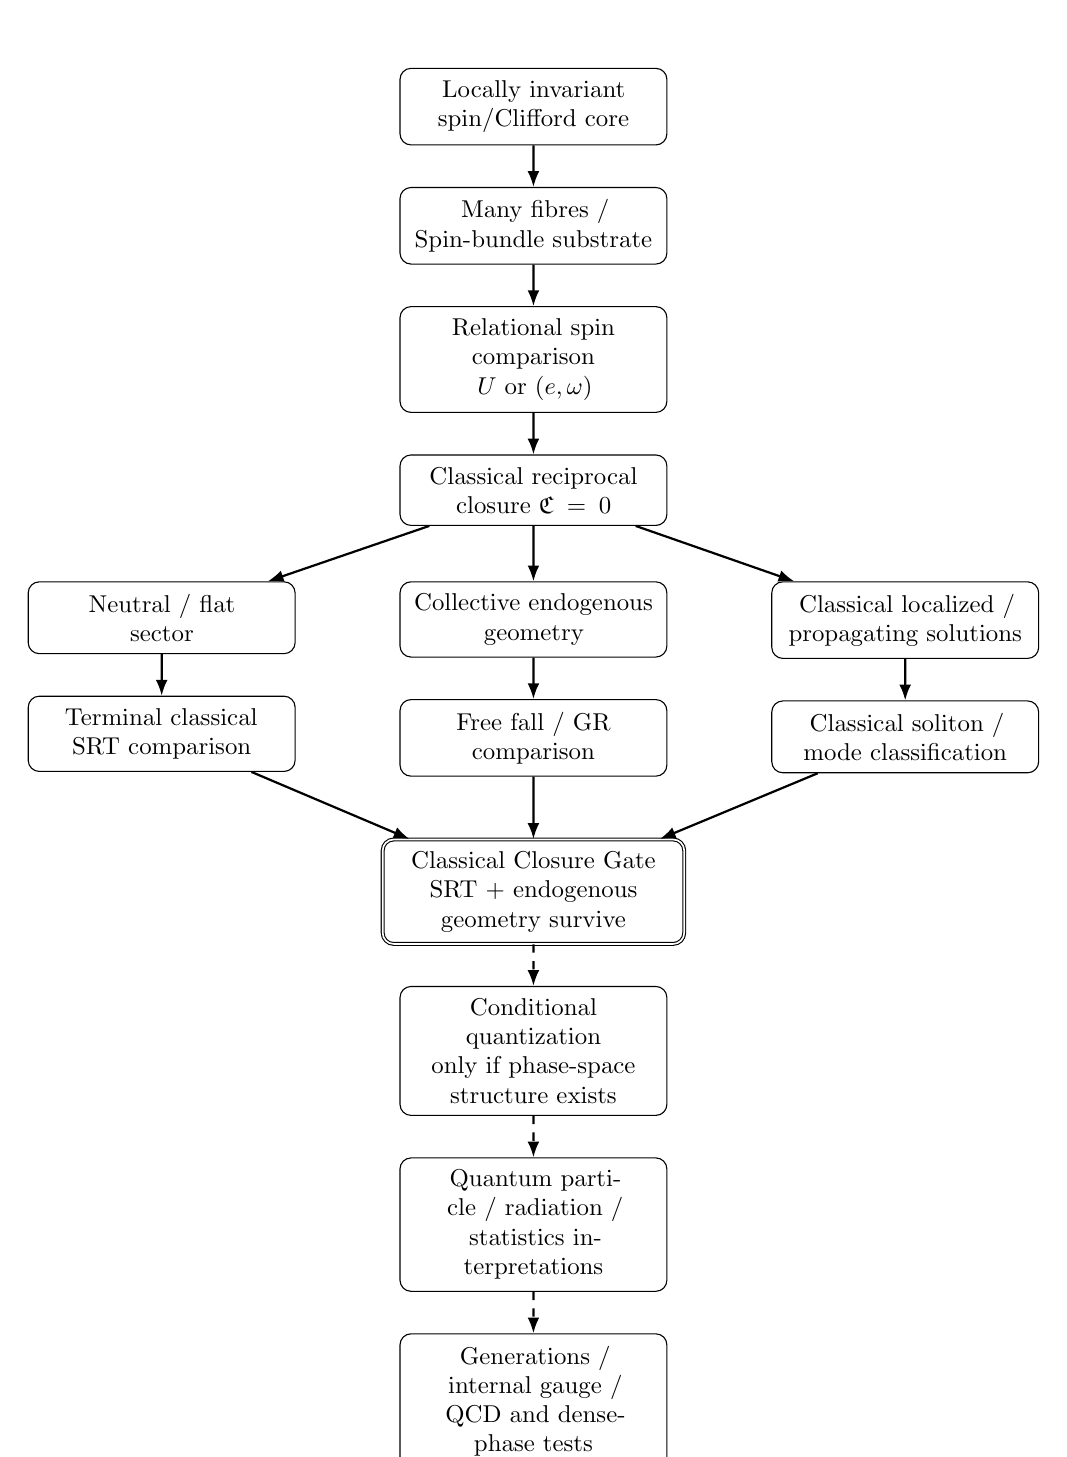
\begin{tikzpicture}[scale=0.88,transform shape,
  node distance=6mm and 9mm,
  box/.style={draw,rounded corners,align=center,inner sep=5pt,text width=35mm},
  gate/.style={draw,double,rounded corners,align=center,inner sep=5pt,text width=40mm},
  arr/.style={-{Latex[length=2mm]},thick},
  darr/.style={-{Latex[length=2mm]},thick,dashed}
]
\node[box] (core) {Locally invariant\\spin/Clifford core};
\node[box,below=of core] (bundle) {Many fibres /\\Spin-bundle substrate};
\node[box,below=of bundle] (rel) {Relational spin comparison\\$U$ or $(e,\omega)$};
\node[box,below=of rel] (closure) {Classical reciprocal\\closure $\mathfrak C=0$};
\node[box,below left=8mm and 15mm of closure] (flat) {Neutral / flat\\sector};
\node[box,below=8mm of closure] (geom) {Collective endogenous\\geometry};
\node[box,below right=8mm and 15mm of closure] (exc) {Classical localized /\\propagating solutions};
\node[box,below=of flat] (srt) {Terminal classical\\SRT comparison};
\node[box,below=of geom] (gr) {Free fall / GR\\comparison};
\node[box,below=of exc] (cmodes) {Classical soliton /\\mode classification};
\node[gate,below=9mm of gr] (qgate) {Classical Closure Gate\\SRT + endogenous geometry survive};
\node[box,below=of qgate] (quant) {Conditional quantization\\only if phase-space structure exists};
\node[box,below=of quant] (qext) {Quantum particle / radiation /\\statistics interpretations};
\node[box,below=of qext] (qcd) {Generations / internal gauge /\\QCD and dense-phase tests};
\draw[arr] (core)--(bundle);
\draw[arr] (bundle)--(rel);
\draw[arr] (rel)--(closure);
\draw[arr] (closure)--(flat);
\draw[arr] (closure)--(geom);
\draw[arr] (closure)--(exc);
\draw[arr] (flat)--(srt);
\draw[arr] (geom)--(gr);
\draw[arr] (exc)--(cmodes);
\draw[arr] (srt)--(qgate);
\draw[arr] (gr)--(qgate);
\draw[arr] (cmodes)--(qgate);
\draw[darr] (qgate)--(quant);
\draw[darr] (quant)--(qext);
\draw[darr] (qext)--(qcd);
\end{tikzpicture}
\end{center}

\begin{remark}[Meaning of the double/dashed boundary]
Everything above the Classical Closure Gate belongs to the core RSCH and is to be formulated and falsified classically.  The dashed branch below the gate is conditional.  Failure of that later quantization branch does not retroactively invalidate a successful classical SRT/geometry closure, whereas success of a quantum extension cannot retroactively repair failure above the gate.
\end{remark}

\section{Failure modes and hard falsifiers}

\begin{falsifier}[No nontrivial closure]
If every gauge-covariant reciprocal closure compatible with the local core is either trivial/pure gauge or requires importing the target dynamical equations, RSCH fails at its central step.
\end{falsifier}

\begin{falsifier}[Two-law failure]
If kinematic response and geometric/free-fall response require irreducibly independent fundamental laws rather than two boundary realizations of one closure, the proposed common mechanism fails.
\end{falsifier}

\begin{falsifier}[Clock-synchronization substitution]
If the construction obtains its core effect only by introducing a preferred clock field, a prescribed simultaneity convention, an external lapse/time slicing, or an absolute temporal phase and then calling that object ``synchronization'', it is not an implementation of RSCH.
\end{falsifier}

\begin{falsifier}[Quantum-rescue failure]
If the classical relational closure fails its existence, reciprocity, SRT or endogenous-geometry tests and the target behaviour appears only after adding quantum postulates or a different quantum dynamical law, the classical RSCH has failed.  The resulting quantum model, if consistent, is a distinct hypothesis rather than a repaired RSCH.
\end{falsifier}

\begin{falsifier}[Local invariance failure]
If fitting observations requires changing the local Minkowski/spin core from fibre to fibre rather than changing relational geometry, the stated hypothesis fails in its present form.
\end{falsifier}

\begin{falsifier}[Scale laundering]
If masses or gravitational couplings appear only because a dimensionful target value was inserted under a renamed parameter or unit convention, the emergence claim fails.
\end{falsifier}

\begin{falsifier}[Matter failure]
If the closure has no stable localized finite-energy solutions, the proposed matter branch fails even if the geometric branch survives.
\end{falsifier}

\begin{falsifier}[Generation failure]
If stable-state classification does not naturally produce the observed generation pattern, the generation extension fails; the geometry hypothesis need not fail with it.
\end{falsifier}

\begin{falsifier}[Strong-sector failure]
If no appropriate internal non-Abelian gauge sector emerges, no claim about confinement or QGP follows from RSCH.  If such a sector emerges but fails asymptotic-freedom/confinement benchmarks, the QCD extension is falsified.
\end{falsifier}

\section{Relationship to established primary literature}

The purpose of this section is to delimit novelty rather than accumulate analogies.

\paragraph{Nakahara (2003, 2nd ed.).}  Nakahara provides a modern textbook control architecture connecting Lorentzian tangent-space metrics, local orthonormal frames/vierbeins, fibre and principal bundles, associated bundles, principal connections, holonomy, curvature, spinorial covariant derivatives, general-relativistic dynamics and the Spin-lift/$w_2$ obstruction \cite{Nakahara2003}.  RSCH uses this source as a \emph{standard-target and dependency check}, not as evidence for the new closure.  In particular, the relations $g=e^*\eta$, $\Omega=\dd\omega+\tfrac12[\omega\wedge\omega]$, the distinction between curvature and torsion, and the geometry-to-spinor covariant coupling are established structures.  The unproved RSCH arrow is the endogenous selection of $(e,\omega)$ from the deeper relational core and state by one reciprocal classical law.

\paragraph{Cartan (1923).}  Affine connections, curvature and torsion are established geometric structures \cite{Cartan1923}.  RSCH does not claim their invention; it asks what selects their physical configuration from the deeper core.

\paragraph{Fock and Weyl (1929).}  Spinors in gravitational/local-frame settings and the need for local frame/connection data are established \cite{Fock1929,Weyl1929}.  RSCH asks whether the relevant coupling structure can be derived from the project's reconstructed dependency chain rather than appended as an external gravitational formalism.

\paragraph{Ambrose--Singer (1953).}  Curvature controls holonomy \cite{AmbroseSinger1953}.  Therefore loop mismatch is a mathematically legitimate probe of non-flat comparison structure.  This theorem does not supply a self-regulation law.

\paragraph{Yang--Mills (1954).}  Local non-Abelian symmetry leads to nonlinear gauge fields \cite{YangMills1954}.  This is a benchmark for any later internal gauge sector, not a reason to identify spin holonomy with colour.

\paragraph{Kibble (1961).}  Localizing the inhomogeneous Lorentz group introduces vierbein and connection variables and provides a gauge-gravity action with spin-dependent torsion effects \cite{Kibble1961}.  This is especially close structurally and therefore an essential control: a purported derivation that merely reconstructs Kibble after assuming his action has not established RSCH.

\paragraph{Milnor and Geroch (1963--1970).}  Global spin structures have topological existence conditions and are additional structure beyond a Lorentz metric \cite{Milnor1963,Geroch1968,Geroch1970}.  These conditions must be formalized before a global relational Spin-comparison programme can legitimately speak of spinor fields on arbitrary manifolds.

\paragraph{Einstein and Schwarzschild (1916).}  General relativity and its exact spherically symmetric exterior solution provide macroscopic geometry benchmarks \cite{Einstein1916,Schwarzschild1916}; they are explicitly forbidden as definitions of the new closure.

\paragraph{Skyrme (1961).}  Finite-energy particle-like nonlinear field configurations provide a primary precedent for emergent localized objects \cite{Skyrme1961}.  RSCH requires its own stability mechanism and observables.

\paragraph{Wilson, Gross--Wilczek, Politzer, Cabibbo--Parisi, Collins--Perry, Shuryak.}  Gauge-invariant confinement, asymptotic freedom, quark liberation/deconfinement and dense/hot quark matter are stringent strong-interaction benchmarks \cite{Wilson1974,GrossWilczek1973,Politzer1973,CabibboParisi1975,CollinsPerry1975,Shuryak1978}.  They belong only to a late branch of the programme.

\section{Conclusion: the hypothesis in one statement}

The research hypothesis can be stated compactly as follows.

\begin{hypothesis}[Condensed form]
There exists a deeper locally invariant spin/Clifford core whose many-fibre relational Spin-comparison data are jointly constrained with the classical local/core state by a single gauge-covariant reciprocal closure.  The fibrewise Minkowski/spin core remains invariant, while the relational background is endogenous.  The standard geometric arrows are not part of the novelty: $e$ induces $g=e^*\eta$, $\omega$ defines parallel transport and curvature, and $(e,\omega)$ define torsion.  The hypothesized new arrow is the endogenous selection of the physically realized $(e,\omega)$ from the relational many-fibre/core state without inserting a known gravitational action.  State-side and geometry-side perturbations are two boundary realizations of the same classical law.  The neutral sector must reproduce special-relativistic kinematics; collective non-flat solutions must generate viable gravitational geometry and free fall without importing the target field equations.  Classical localized and propagating solutions may then be classified.  Quantization is not part of the defining hypothesis and may be attempted only after the classical closure survives its SRT and geometry gates and supplies a suitable phase-space/Hamiltonian or symplectic structure.  Quantum assumptions may not be used to rescue failure of the classical closure.  Mass, quantum-particle interpretations, generations and strong-interaction phases are later invariants or extension tests, and every dimensionful scale must have explicit provenance.
\end{hypothesis}

The decisive mathematical unknown is therefore not ``what is curvature?'' but
\begin{center}
\fbox{\parbox{0.90\linewidth}{\centering
What is the minimal native \emph{classical} relational spin closure $\mathfrak C$ that makes local/core state and relational geometry mutually self-consistent across many invariant fibres?}}
\end{center}
If no such nontrivial classical closure exists, the core programme terminates at that point.  If one exists, the SRT and gravitational comparisons remain independent classical falsification stages.  Only after both have survived may a quantization branch be opened, and only if a suitable classical phase-space structure exists.  Matter, radiation, particle, generation and QCD interpretations are still later tests rather than guarantees.  This ordering is essential: neither known classical target equations nor known quantum postulates may be inserted backwards into the premises.

\clearpage
\begin{thebibliography}{99}

\bibitem{TaoAccurate}
T. Tao,
\emph{Describe the results accurately}, in Advice on Writing Papers, What's New (2007).
\url{https://terrytao.wordpress.com/advice-on-writing-papers/describe-the-results-accurately/}.

\bibitem{Nakahara2003}
M. Nakahara,
\emph{Geometry, Topology and Physics}, 2nd ed.,
Graduate Student Series in Physics, Institute of Physics Publishing, Bristol and Philadelphia (2003).
Relevant control sections: 7.4--7.5, 7.8, 7.10.3, 9.1--9.4, 10.1--10.4, and 11.6.
ISBN: 0-7503-0606-8.

\bibitem{Cartan1923}
E. Cartan,
\emph{Sur les variétés à connexion affine et la théorie de la relativité généralisée (première partie)},
Annales scientifiques de l'École Normale Supérieure, 40 (1923), 325--412.
DOI: \href{https://doi.org/10.24033/asens.751}{10.24033/asens.751}.

\bibitem{Fock1929}
V. Fock,
\emph{Geometrisierung der Diracschen Theorie des Elektrons},
Zeitschrift für Physik 57 (1929), 261--277.
DOI: \href{https://doi.org/10.1007/BF01339714}{10.1007/BF01339714}.

\bibitem{Weyl1929}
H. Weyl,
\emph{Gravitation and the Electron},
Proceedings of the National Academy of Sciences 15(4) (1929), 323--334.
DOI: \href{https://doi.org/10.1073/pnas.15.4.323}{10.1073/pnas.15.4.323}.

\bibitem{AmbroseSinger1953}
W. Ambrose and I. M. Singer,
\emph{A Theorem on Holonomy},
Transactions of the American Mathematical Society 75(3) (1953), 428--443.
DOI: \href{https://doi.org/10.1090/S0002-9947-1953-0063739-1}{10.1090/S0002-9947-1953-0063739-1}.

\bibitem{YangMills1954}
C. N. Yang and R. L. Mills,
\emph{Conservation of Isotopic Spin and Isotopic Gauge Invariance},
Physical Review 96 (1954), 191--195.
DOI: \href{https://doi.org/10.1103/PhysRev.96.191}{10.1103/PhysRev.96.191}.

\bibitem{Kibble1961}
T. W. B. Kibble,
\emph{Lorentz Invariance and the Gravitational Field},
Journal of Mathematical Physics 2(2) (1961), 212--221.
DOI: \href{https://doi.org/10.1063/1.1703702}{10.1063/1.1703702}.

\bibitem{Skyrme1961}
T. H. R. Skyrme,
\emph{A Non-Linear Field Theory},
Proceedings of the Royal Society A 260 (1961), 127--138.
DOI: \href{https://doi.org/10.1098/rspa.1961.0018}{10.1098/rspa.1961.0018}.

\bibitem{Milnor1963}
J. Milnor,
\emph{Spin Structures on Manifolds},
L'Enseignement Mathématique 9 (1963), 198--203.
Persistent DOI record: \href{https://doi.org/10.5169/seals-38784}{10.5169/seals-38784}.

\bibitem{Geroch1968}
R. Geroch,
\emph{Spinor Structure of Space-Times in General Relativity. I},
Journal of Mathematical Physics 9 (1968), 1739--1744.
DOI: \href{https://doi.org/10.1063/1.1664507}{10.1063/1.1664507}.

\bibitem{Geroch1970}
R. Geroch,
\emph{Spinor Structure of Space-Times in General Relativity. II},
Journal of Mathematical Physics 11 (1970), 343--348.
DOI: \href{https://doi.org/10.1063/1.1665067}{10.1063/1.1665067}.

\bibitem{Einstein1916}
A. Einstein,
\emph{Die Grundlage der allgemeinen Relativitätstheorie},
Annalen der Physik 354(7) (1916), 769--822.
DOI: \href{https://doi.org/10.1002/andp.19163540702}{10.1002/andp.19163540702}.

\bibitem{Schwarzschild1916}
K. Schwarzschild,
\emph{Über das Gravitationsfeld eines Massenpunktes nach der Einsteinschen Theorie},
Sitzungsberichte der Königlich Preussischen Akademie der Wissenschaften (1916), 189--196.
Primary scan (SAO/NASA ADS): \url{https://adsabs.harvard.edu/pdf/1916SPAW.......189S}.

\bibitem{Wilson1974}
K. G. Wilson,
\emph{Confinement of Quarks},
Physical Review D 10 (1974), 2445--2459.
DOI: \href{https://doi.org/10.1103/PhysRevD.10.2445}{10.1103/PhysRevD.10.2445}.

\bibitem{GrossWilczek1973}
D. J. Gross and F. Wilczek,
\emph{Ultraviolet Behavior of Non-Abelian Gauge Theories},
Physical Review Letters 30 (1973), 1343--1346.
DOI: \href{https://doi.org/10.1103/PhysRevLett.30.1343}{10.1103/PhysRevLett.30.1343}.

\bibitem{Politzer1973}
H. D. Politzer,
\emph{Reliable Perturbative Results for Strong Interactions?},
Physical Review Letters 30 (1973), 1346--1349.
DOI: \href{https://doi.org/10.1103/PhysRevLett.30.1346}{10.1103/PhysRevLett.30.1346}.


\bibitem{CabibboParisi1975}
N. Cabibbo and G. Parisi,
\emph{Exponential Hadronic Spectrum and Quark Liberation},
Physics Letters B 59(1) (1975), 67--69.
DOI: \href{https://doi.org/10.1016/0370-2693(75)90158-6}{10.1016/0370-2693(75)90158-6}.

\bibitem{CollinsPerry1975}
J. C. Collins and M. J. Perry,
\emph{Superdense Matter: Neutrons or Asymptotically Free Quarks?},
Physical Review Letters 34 (1975), 1353--1356.
DOI: \href{https://doi.org/10.1103/PhysRevLett.34.1353}{10.1103/PhysRevLett.34.1353}.


\bibitem{Shuryak1978}
E. V. Shuryak,
\emph{Quark-Gluon Plasma and Hadronic Production of Leptons, Photons and Psions},
Physics Letters B 78(1) (1978), 150--153.
DOI: \href{https://doi.org/10.1016/0370-2693(78)90370-2}{10.1016/0370-2693(78)90370-2}.

\end{thebibliography}

\end{document}
